% !TEX root = ../main.tex


\section{Validation}
\label{sec:validation}

One of the attractions of `run to completion' style modelling languages such as \SCXML is their execution semantics which provides a method for animating models to validate their behaviour.
Our approach to \SCXML refinement results in a single \SCXML final model which can be animated using the existing \SCXML animation tools.
However, we would like to validate the developing \UMLB model at intermediate refinement levels. 
\ColinComment{why? Is it not sufficient to animate the \SCXML}

In previous work~\cite{snook20JSA} we have developed a scenario-based approach to formal modelling using abstract scenarios to validate abstract models.
The method is supported by a `Scenario Checker' tool, based on the \PROB model checker, that allows scenarios to be recorded and then replayed to check that important state has not changed since the original run of the scenario.
The Scenario Checker supports the concept of a controller executing a process in response to changes in the environment which is similar to the run to completion concept addressed in our work here.
Events may be annotated as \emph{internal} to indicate that, when enabled, they should be fired automatically until none remain.
Internal events may also be prioritised to give a simple representation of process order in the controller (even if it is left non-deterministic in the model).
The user only has to select external events that trigger the controllers responses.
Since our \SCXML derived models already contain an implementation of run to completion the support provided by the Scenario Checker is sufficient to validate this behaviour.
If desired, internal variables that represent the controllers processing (e.g. the variables that model the \SCXML run to completion variables) can be annotated as \emph{private} so that only the application state is checked during replay.
To help visualise the state of the model, the generated \UMLB state-machine is animated during the scenario validation.

In Figure~\ref{fig:scenarioChecker_recording_drone1} we show a scenario being recorded.



 played back on the drone model.
The main (top-left) editing view shows the state-machine being animated; the model is currently in the fly state.
The bottom left view is the scenario checker control panel.
The top button shows that a pre-recorded scenario is being played back and beside it the enabled external operations are greyed out since manual selection is disabled during playback.
The main button to be used is the \emph{Big Step} button which fires the next step of the scenario.
The bottom-right view shows the history, listing the operations that have already been played.
This is the same as the \PROB history view (top-right), but organises operations into big step runs (an external followed by a sequence of internal operations.
The bottom-middle view shows the state of the main variables and compares to the state when the scenario was recorded.
In the example, a discrepancy has been detected since non-determinism in the raised triggers allowed |DESCEND| to be reached when the scenario was recorded, but the playback has chosen to enter |FLY| instead.


\begin{figure}[!h]
	\centering
	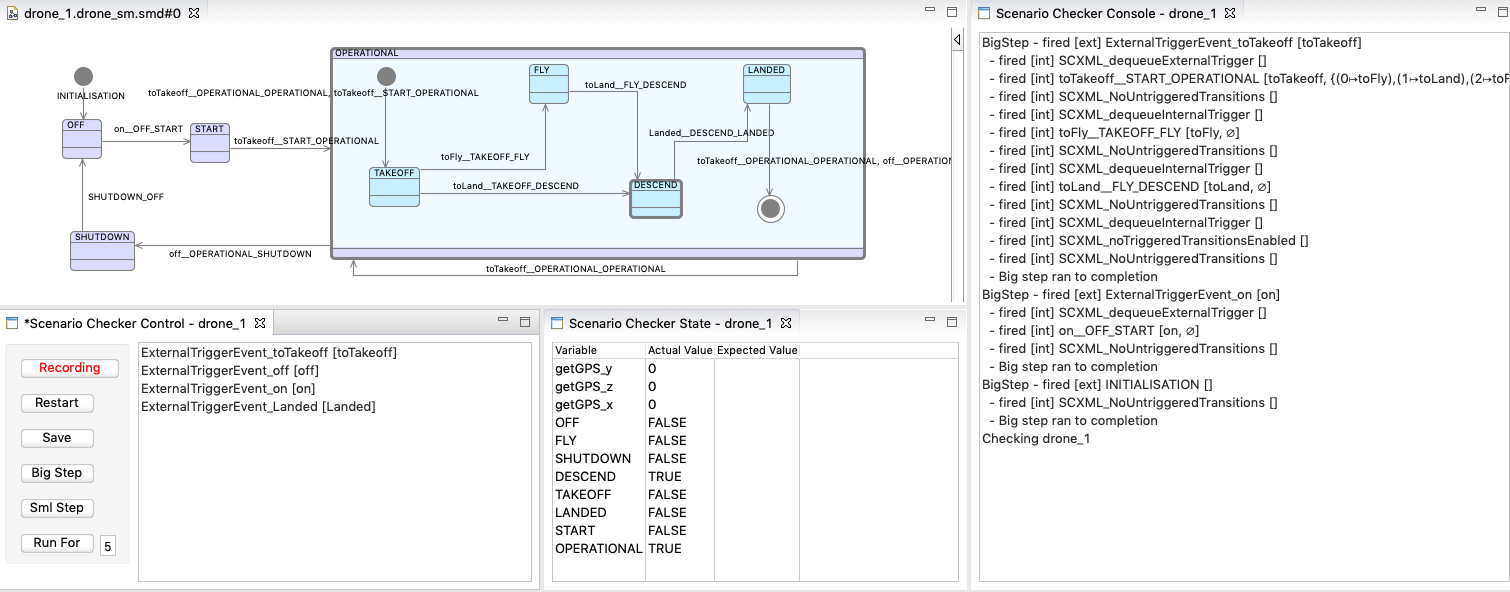
\includegraphics[width=0.90\textwidth, trim=30 50 60 0]{figures/scenarioChecker_recording_drone1.png}
	\caption{Using Scenario Checker to validate behaviour}
	\label{fig:scenarioChecker_recording_drone1}
\end{figure}

While the scenario checker allows us to animate the expected run to completion behaviour, recall that, unless the transitions have all been finalised (i.e. no further refinement is permitted),  other behaviours are possible due to the non-deterministic completion incorporated in case transition guards are later strengthened. 
\ColinInlineComment{To explore these behaviours, we can animate the main version of the machine (i.e. not the special version without non-determinstic features}
%The scenario checker allows the run to completion (i.e. internal events) to be overridden in order to explore these behaviours at an abstract level.
 

%%% Local Variables:
%%% mode: latex
%%% TeX-master: "../main"
%%% End:
